\chapter{Diseño}

\section{Diagramas de clases}

\subsection{Paquete Application}

\begin{figure}[H]
	\centering
	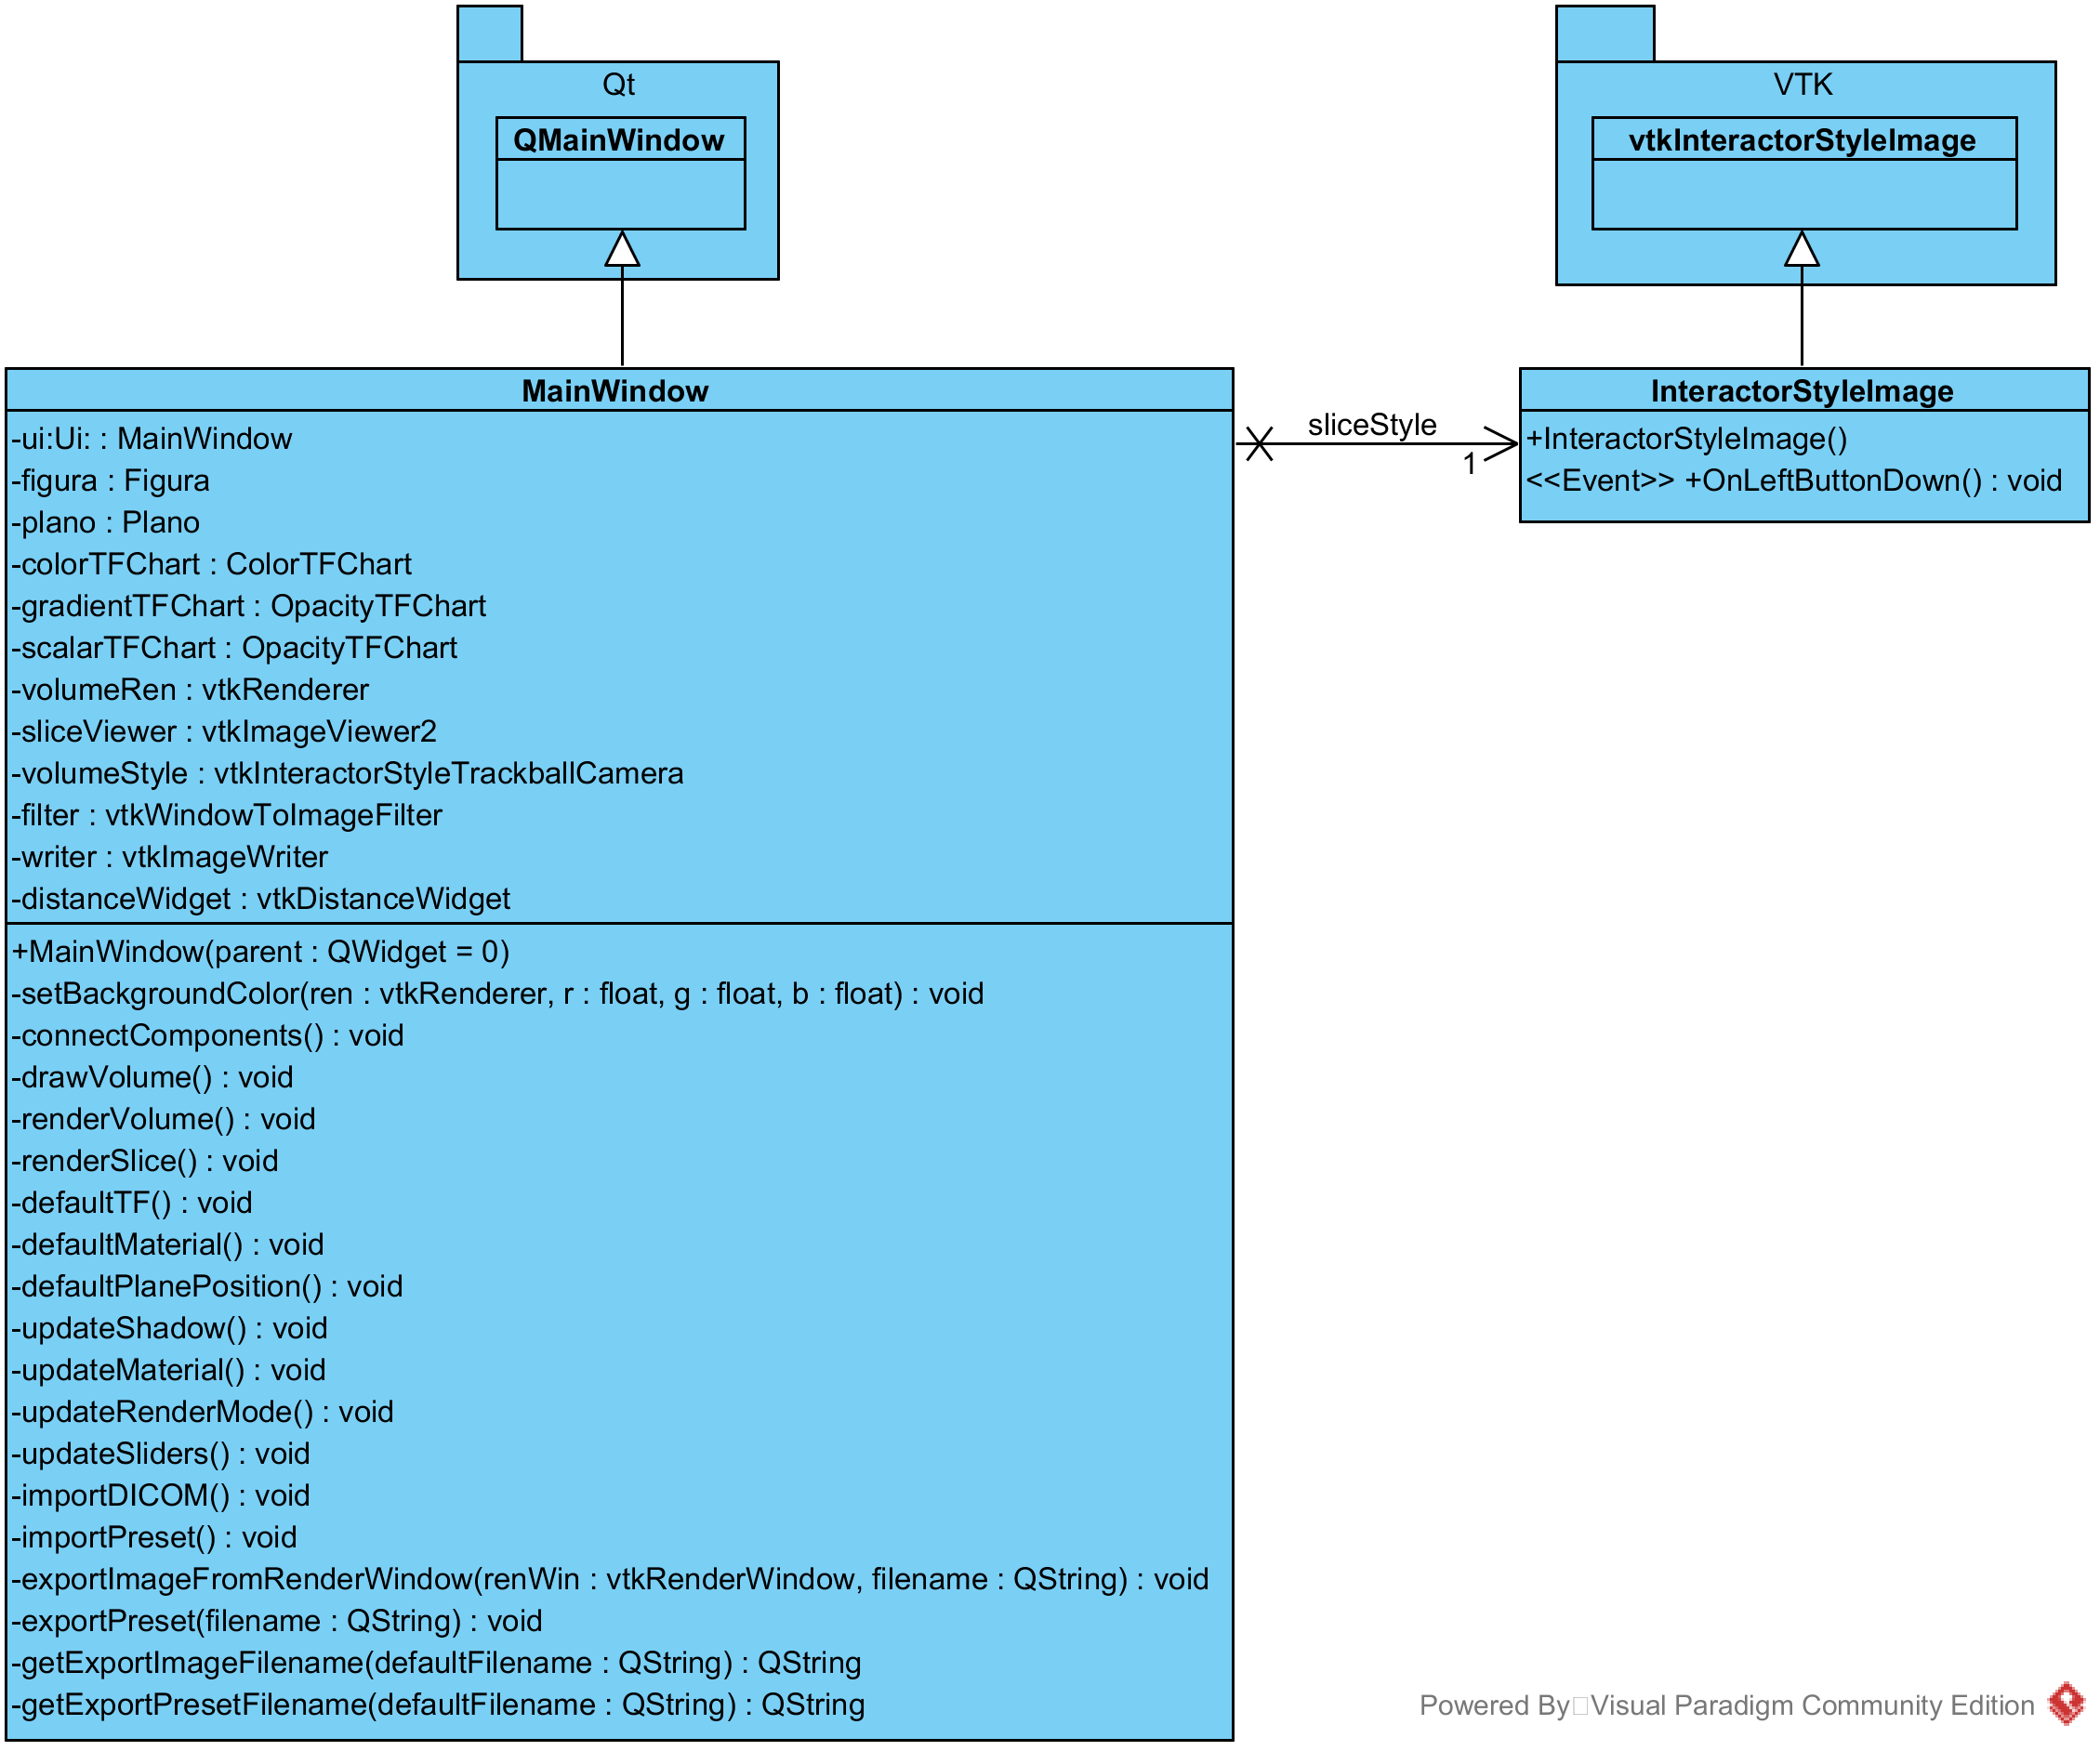
\includegraphics[width=12.5cm]{imagenes/diagramas/application}
	\caption{Diagrama de clases del paquete \textit{Application}}
	\label{fig:diagrama_clases_application}
\end{figure}

\subsection{Paquete Charts}

\begin{figure}[H]
	\centering
	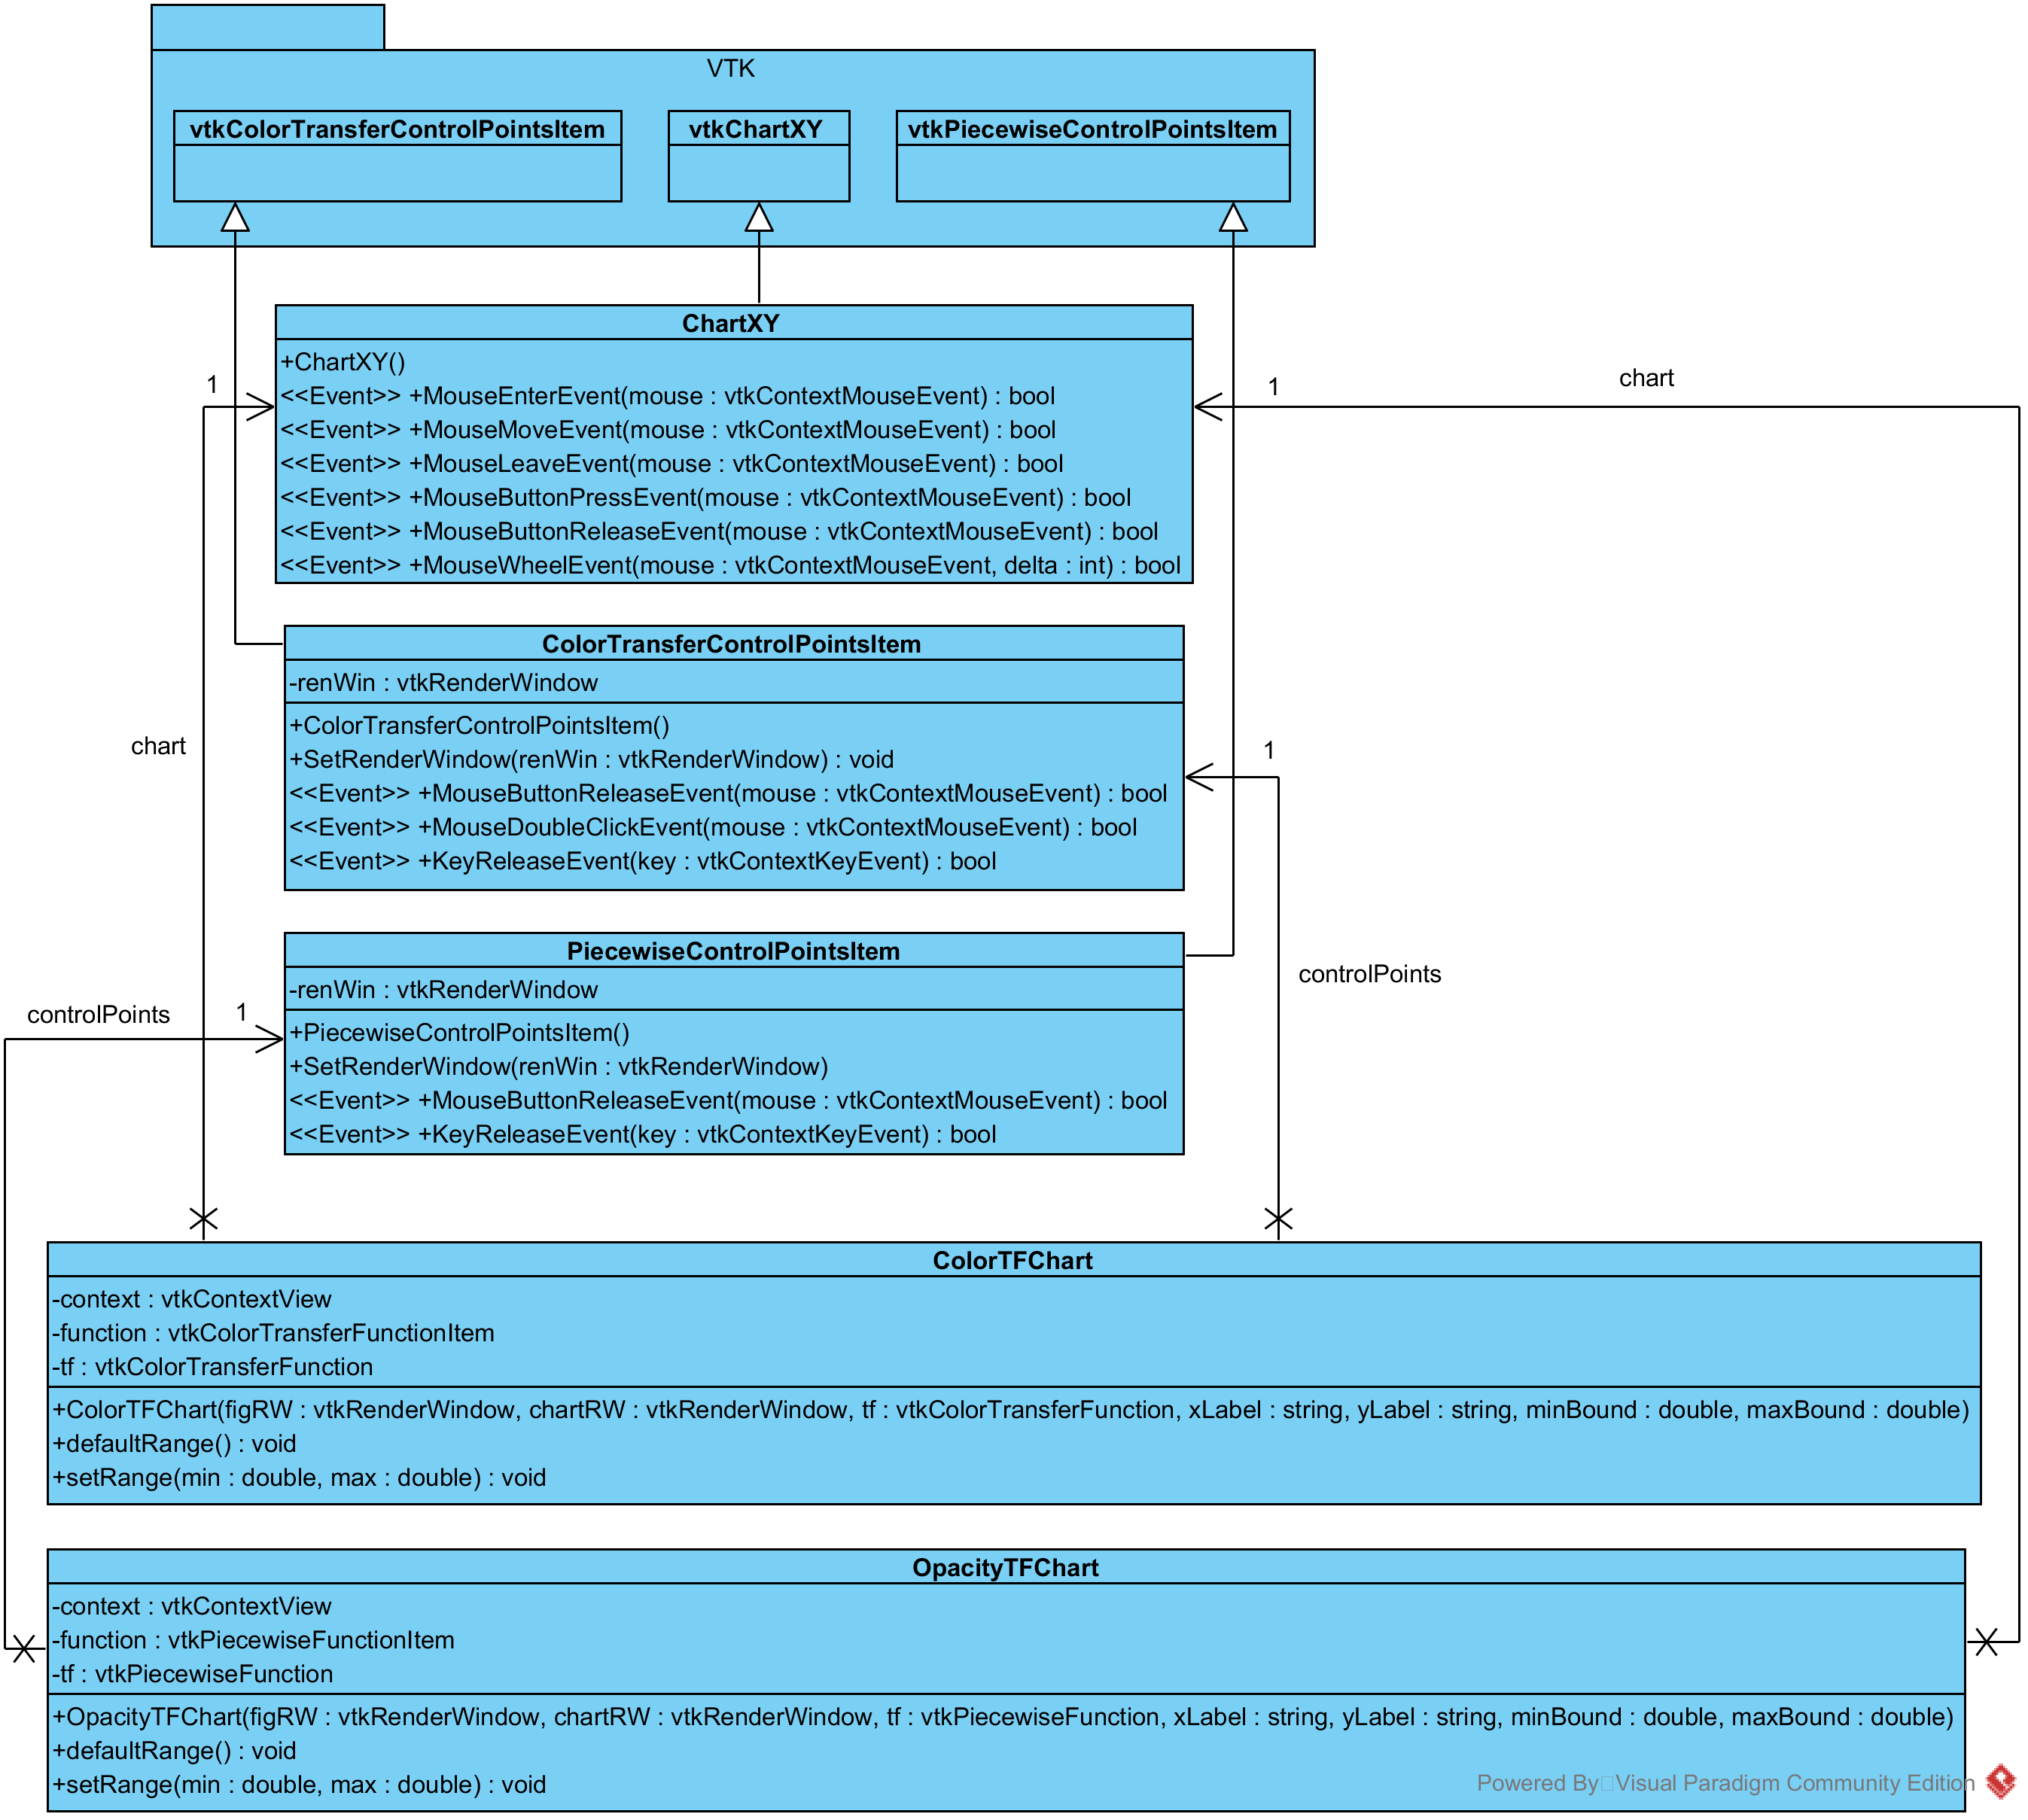
\includegraphics[width=12.5cm]{imagenes/diagramas/charts}
	\caption{Diagrama de clases del paquete \textit{Charts}}
	\label{fig:diagrama_clases_charts}
\end{figure}

\subsection{Paquete Volume}

\begin{figure}[H]
	\centering
	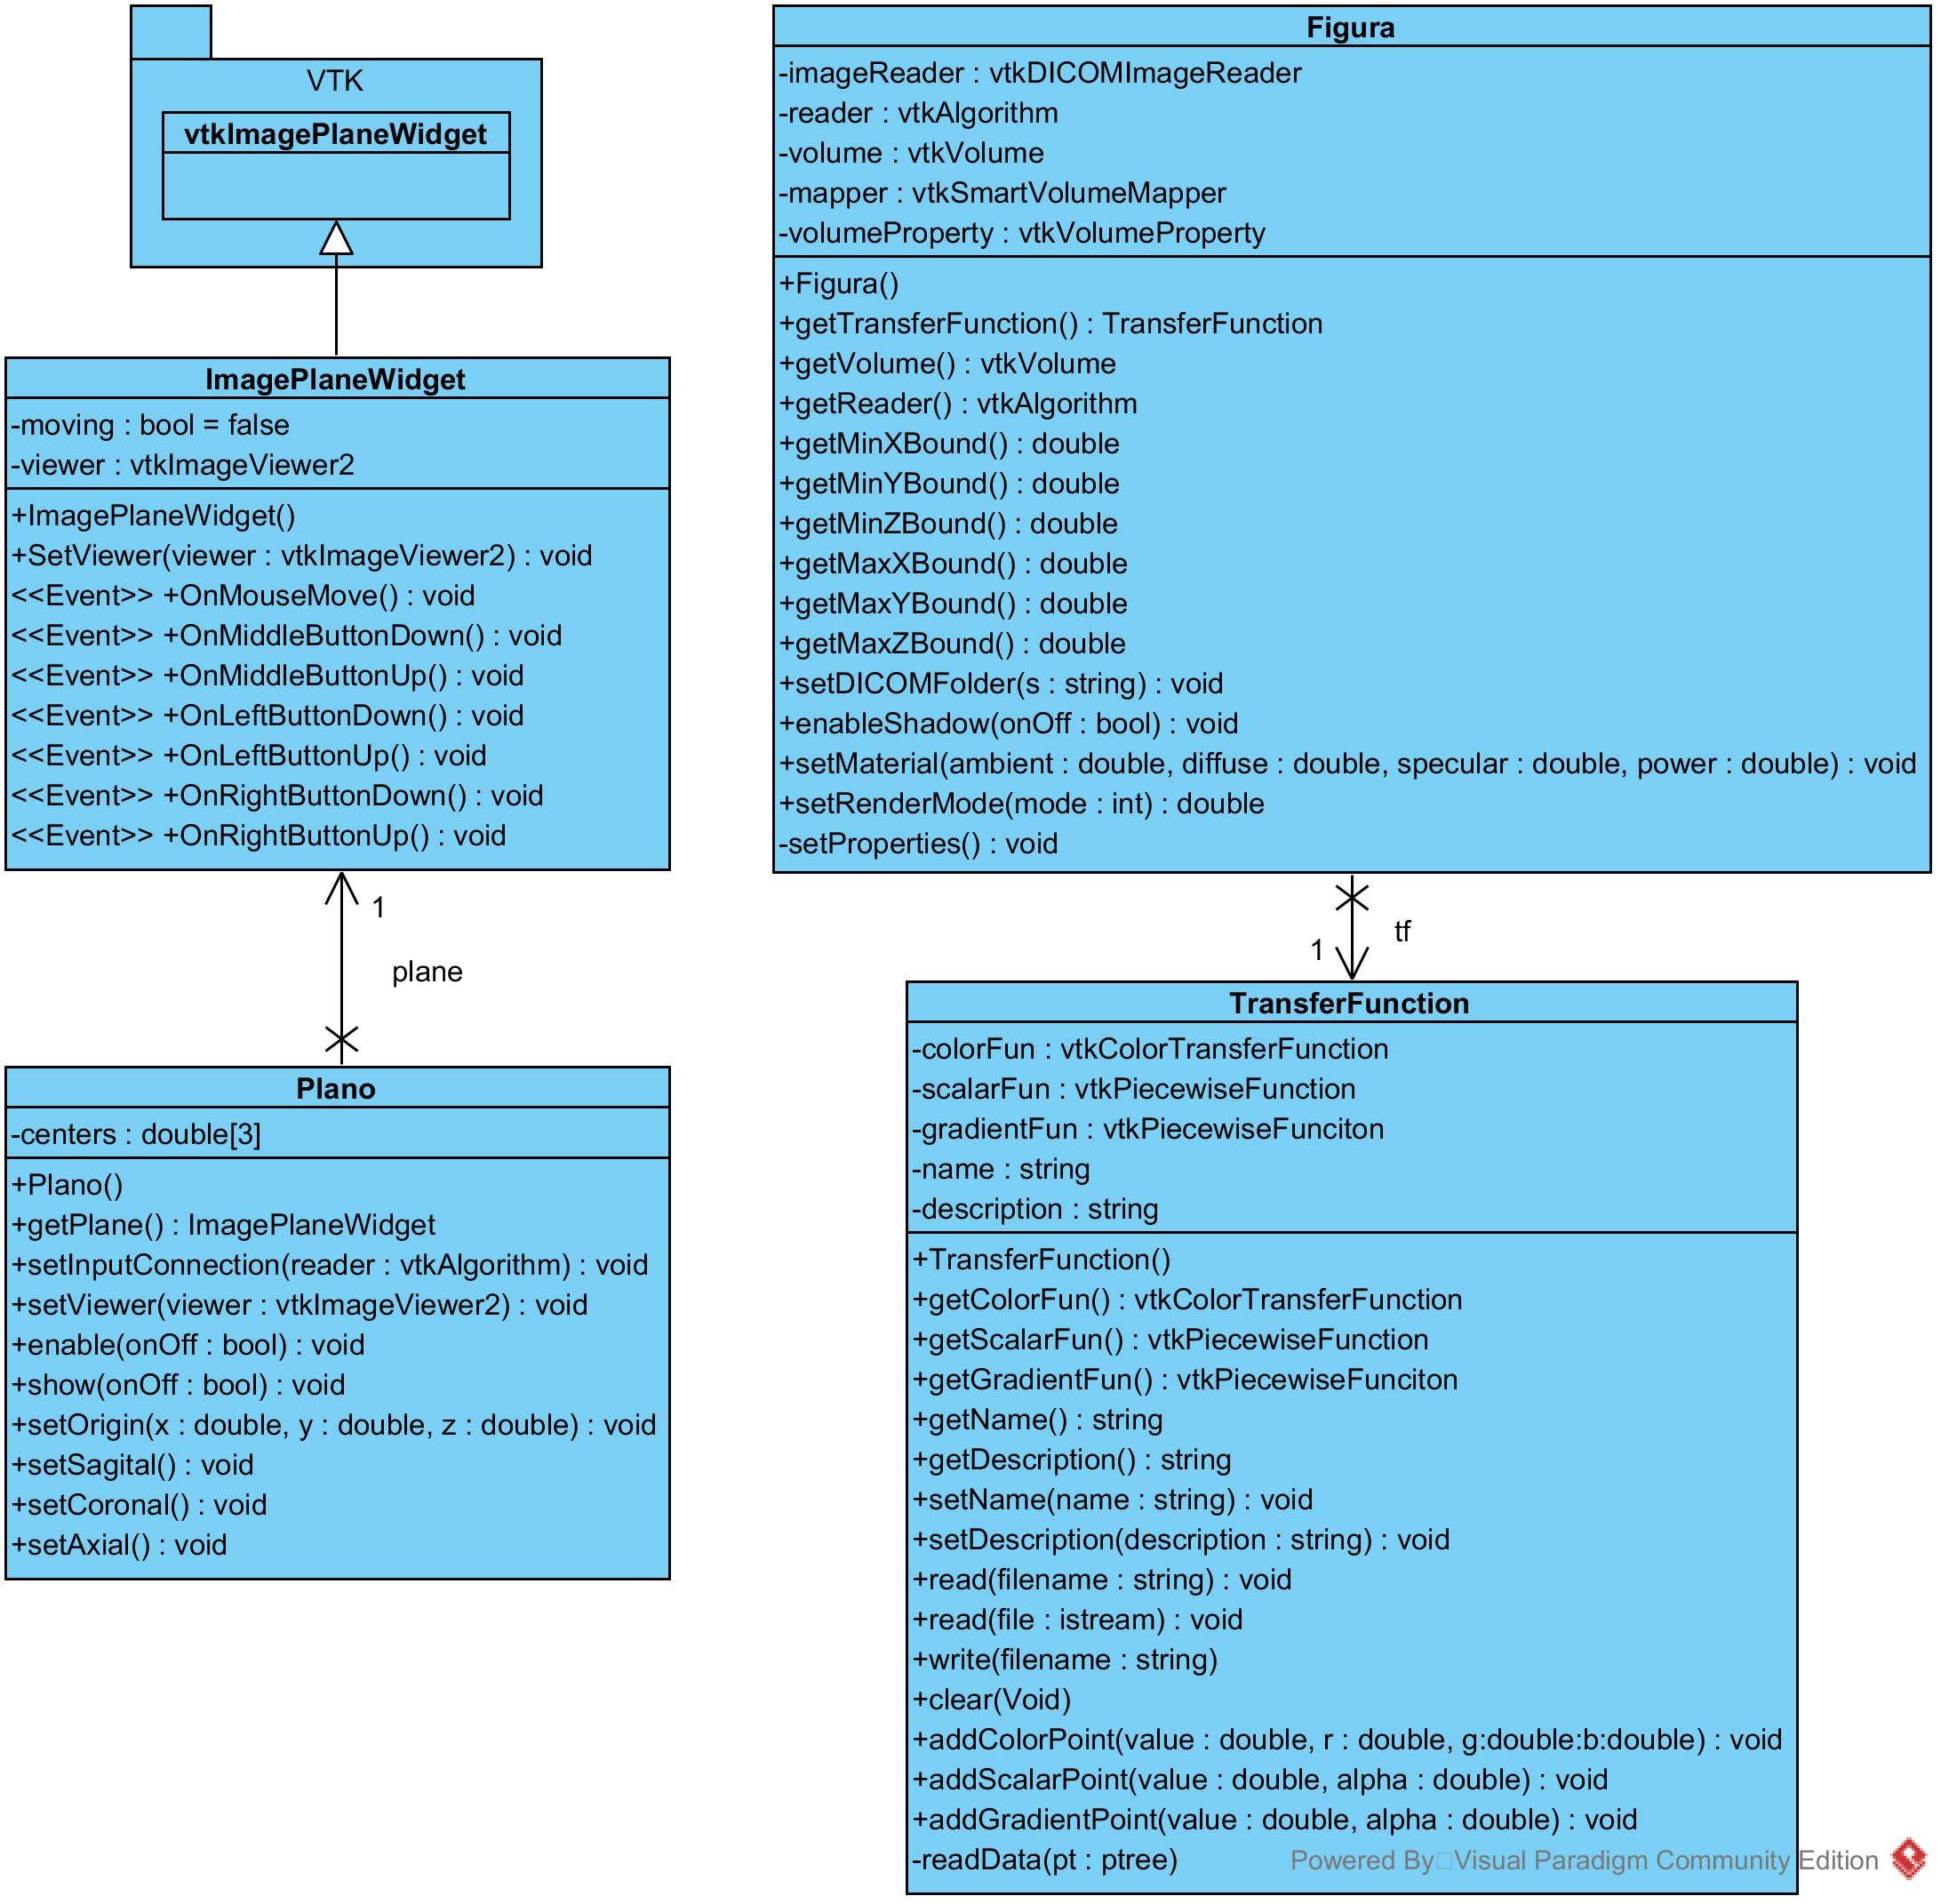
\includegraphics[width=12.5cm]{imagenes/diagramas/volume}
	\caption{Diagrama de clases del paquete \textit{Volume}}
	\label{fig:diagrama_clases_volume}
\end{figure}